A non-anthropomorphic robotic platform was created to limit the influence of shape on the participants' perception. The robotic platform is holonomic and it included Odroid U3 and Arduino Due as processors, 3 metal gear motors with 64 CPR encoders, and omniwheels. Arduino Due is in charge to interface motors, and Odroid U3 hosts the Emotion Enrichment System described here below.
The platform is shown in Figure~\ref{fig:Robot}.

\begin{figure}[t]
\centering%
\subfigure {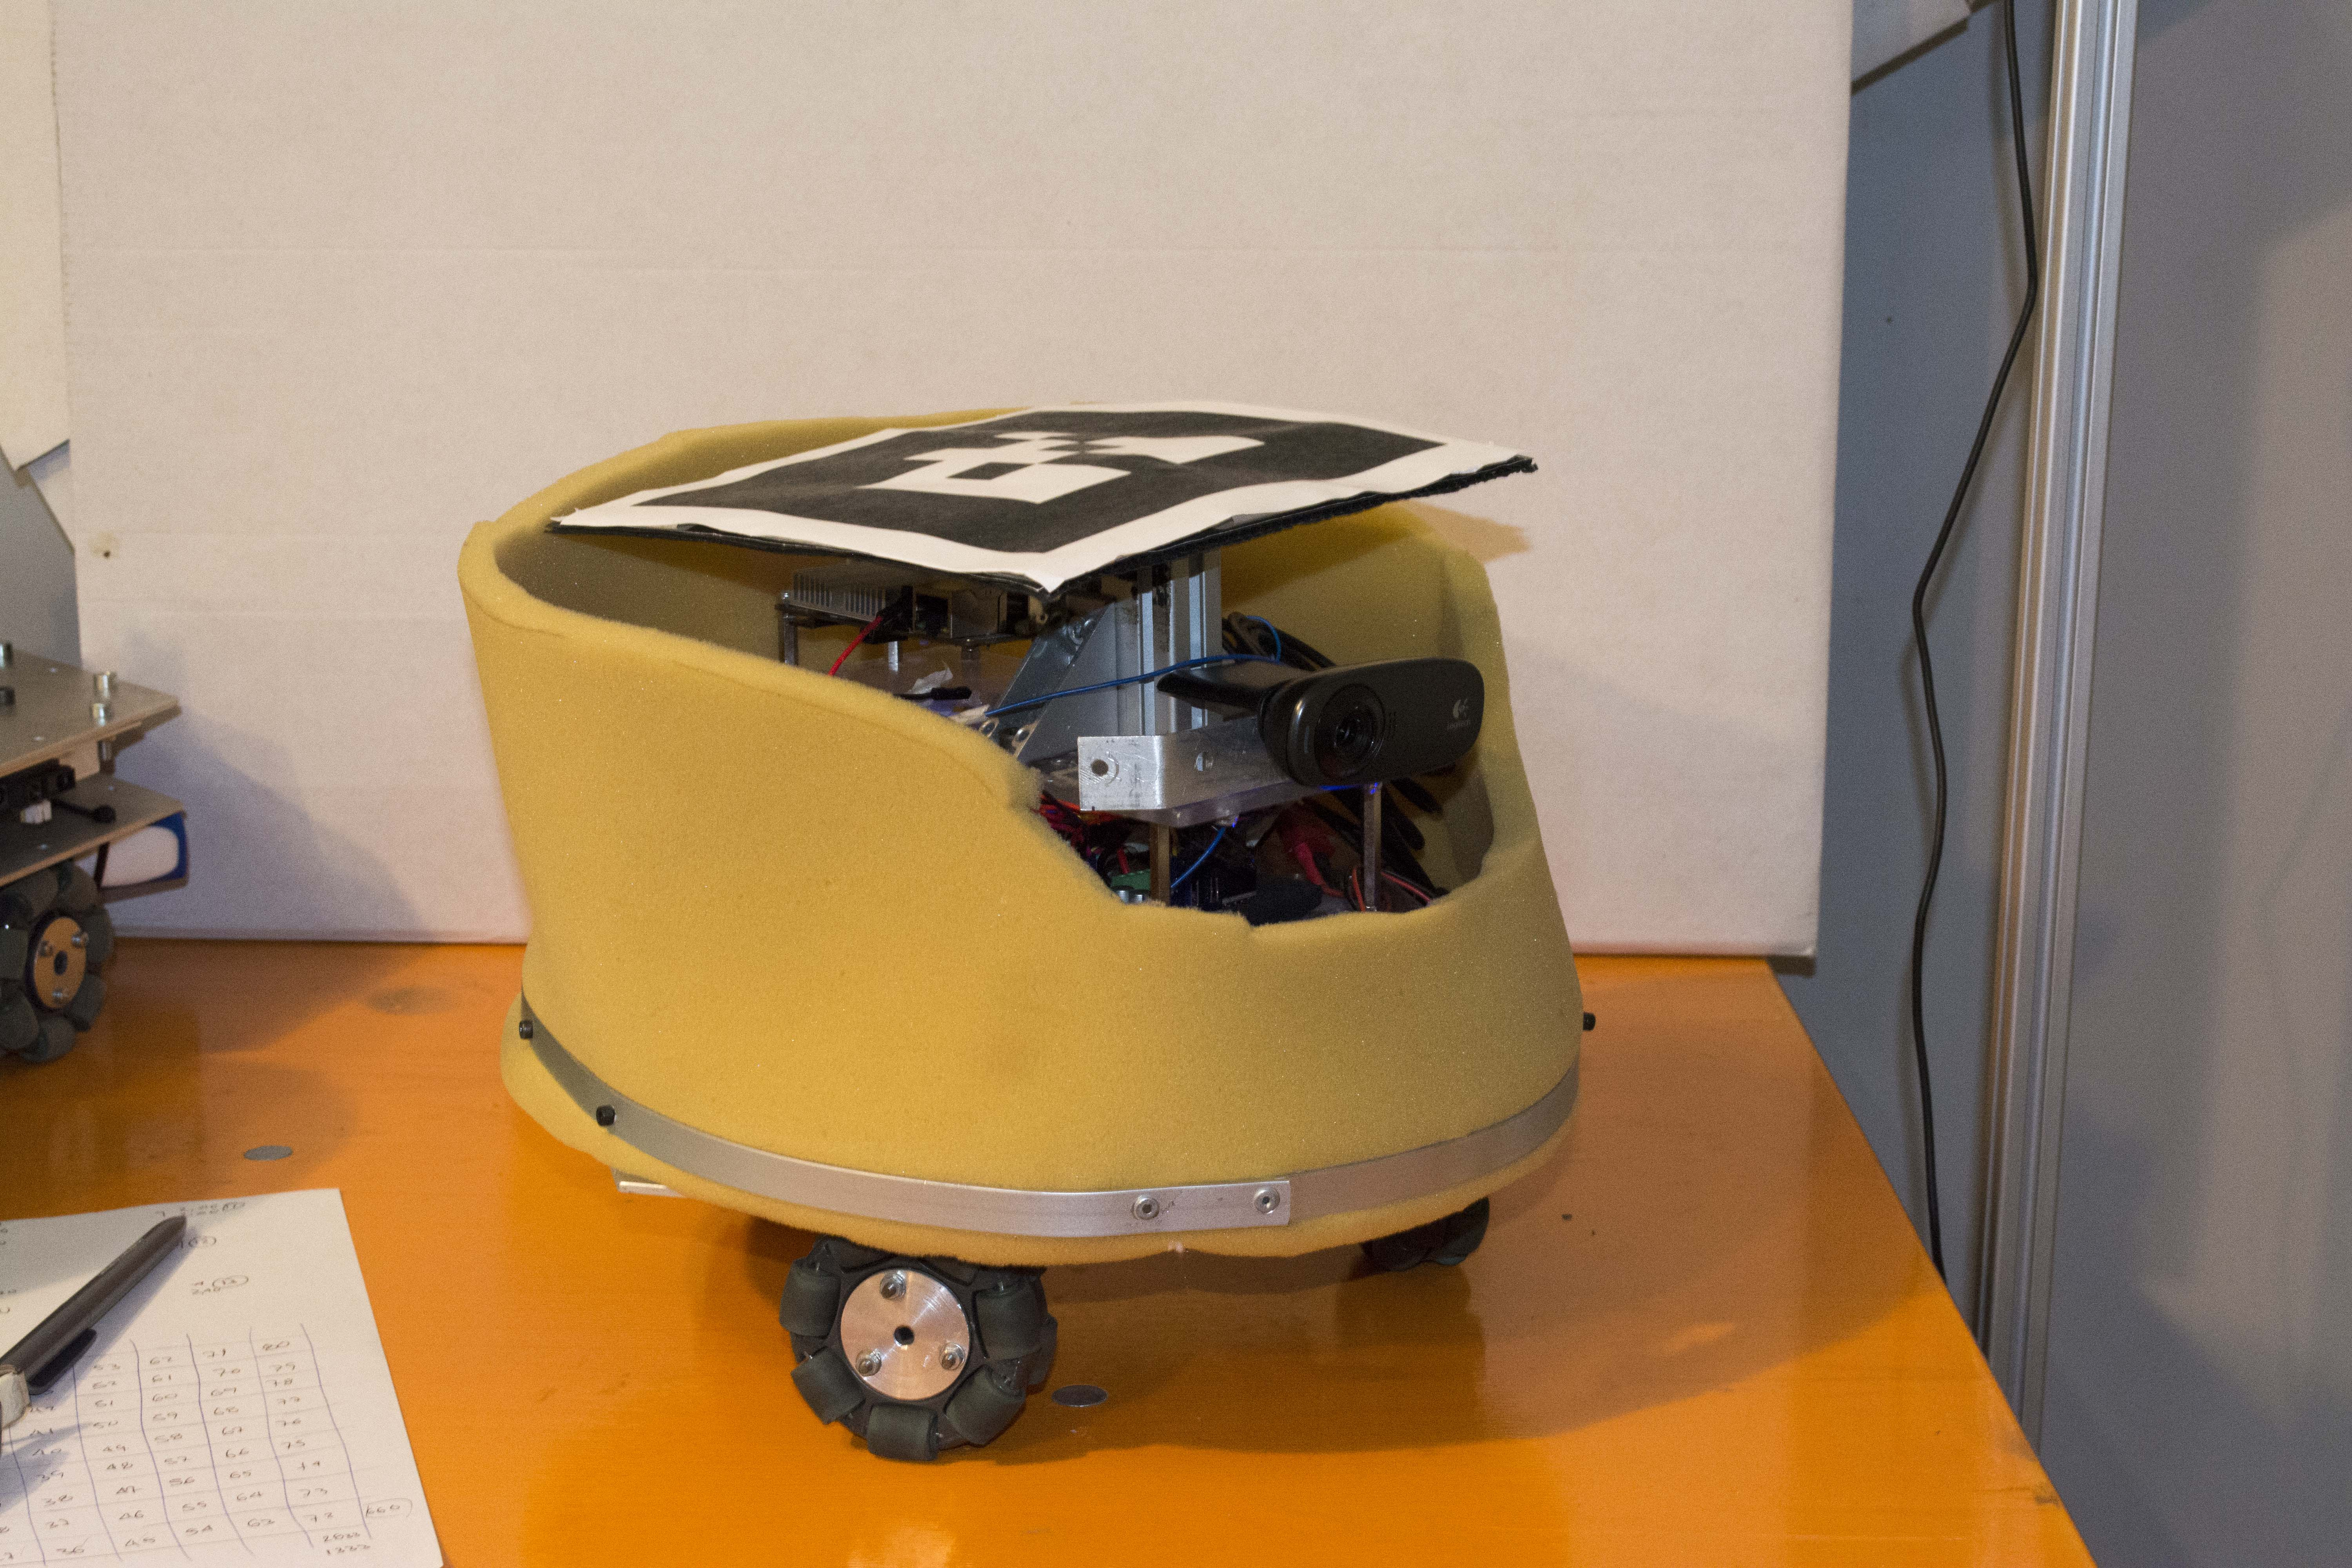
\includegraphics[height=3cm]{./Images/DSC_0447.JPG}}
\hspace{2mm}
\subfigure{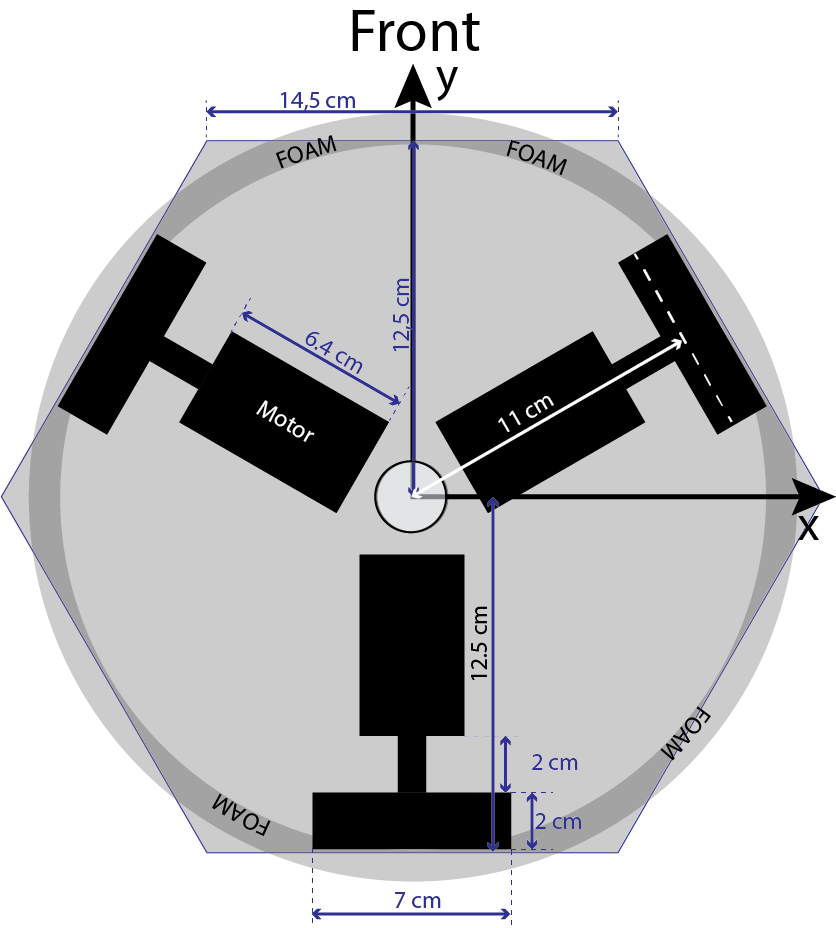
\includegraphics[height=3cm]{./Images/TriskarThird.png}}
\caption{Platform used in the case study (left), and holonomics's blue prints (right). The arrows represent robot's frame of reference.
\label{fig:Robot}}
\end{figure}

An Emotional Enrichment System was designed and implemented to automatize the process of emotion expression~\cite{Angel2017}. It is intended to provide an emotional expression to an action decided a priori, e.g., by the planner. It modifies actions' parameters and adds actions to create the illusion of emotion expression in a robot. To achieve this, the system receives two messages. One message describes actions and the order in which they should be executed. These actions could be executed in parallel, sequentially or as a combination of both. This kind of representation enables the possibility to set up several actions in one message. The other message tells the system the emotion to be expressed and its intensity. These two messages could arrive asynchronously and without any particular order. Every time a message is received, the system updates the robot movements to convey the desired emotion in the specific action.
